\documentclass{article}
\usepackage[margin=0.75in]{geometry}
\usepackage{tabularx}
\usepackage{multirow}
\usepackage{pgfplots}
\pgfplotsset{compat=1.18}
\usepackage[svgnames]{xcolor}
\usepackage{siunitx}
\usepackage{booktabs}
\usepackage{array}
\usepackage{caption}
\usepackage{float}
\usepackage{tikz}
\usepackage{helvet}
\renewcommand{\familydefault}{\sfdefault}

\begin{document}

%--- Corporate 3‑box header ----------------------------------------------------
\begin{center}
\begin{tabularx}{\textwidth}{|>{\centering\arraybackslash}X|>{\centering\arraybackslash}X|>{\centering\arraybackslash}X|}
\hline
\textbf{Company Logo} & \textbf{Annual Steel Production Report} & \textbf{Date: \today} \\
\hline
\end{tabularx}
\end{center}
\vspace{1em}

%--- Section ------------------------------------------------------------------
\section*{Worldwide production of steel}

\paragraph{} This chart shows the six largest producers by nation in 2012. China by far is the worlds largest producer of crude steel.

\paragraph{} Without steel we would have a different world economy.

\paragraph{} No: Railroads? Skyscrapers? Large bridges? Massive ships? Pipe lines?

%--- Bar chart ---------------------------------------------------------------
\begin{figure}[H]
\centering
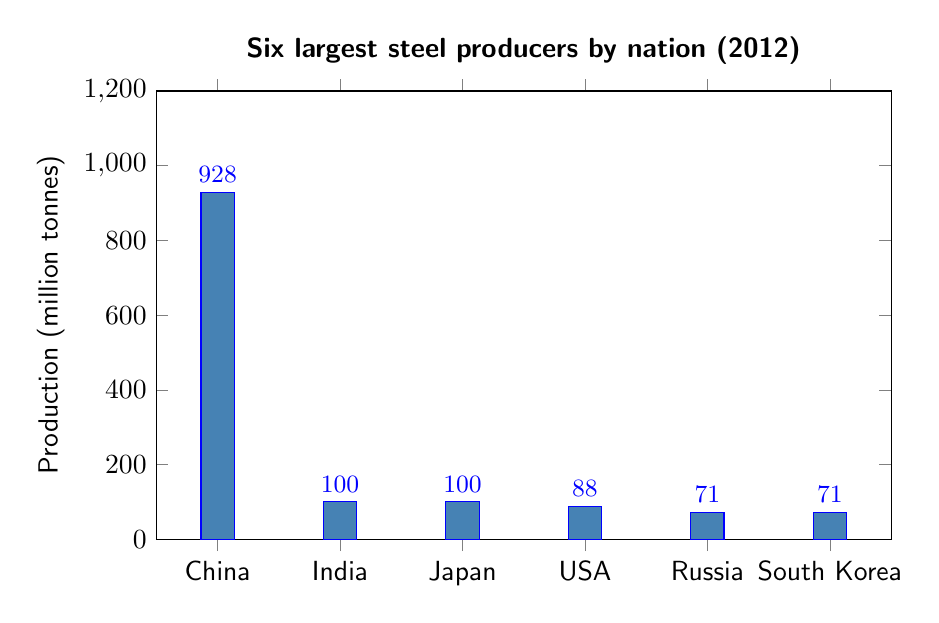
\begin{tikzpicture}
\begin{axis}[
    ybar,
    bar width=12pt,
    width=0.9\textwidth,
    height=0.6\textwidth,
    ylabel={Production (million tonnes)},
    symbolic x coords={China,India,Japan,USA,Russia,South~Korea},
    xtick=data,
    nodes near coords,
    every node near coord/.append style={font=\small},
    ymin=0,
    ymax=1200,
    title={Six largest steel producers by nation (2012)},
    title style={font=\bfseries},
]
\addplot+[fill=SteelBlue] coordinates {
    (China,928) (India,100) (Japan,100) (USA,88) (Russia,71) (South~Korea,71)
};
\end{axis}
\end{tikzpicture}
\caption{Bar chart comparing crude steel production of the six leading nations in 2012. Numerical values are illustrative.}
\end{figure}

\end{document}